% ============================================================================
% COMPLÉMENTS — SPECTRES, GABARITS, REPLIEMENT ET DOUBLE FILTRE RC
% Reprise des sections 5, 6.3, 6.4, 6.13, 7.8 et 7.9 du document source.
% ============================================================================

\clearpage
\section{Compléments sur les spectres et le filtrage}\label{sec:elec-complements-spectres-filtrage}

\subsection{Lire et construire un spectre en amplitude}\label{sec:elec-spectres-exemples}

Pour un signal périodique de fréquence fondamentale $f_0$, le spectre est constitué de raies aux fréquences
\[
0,\quad f_0,\quad 2f_0,\quad 3f_0,\ldots
\]
La raie à $f=0$ représente la valeur moyenne. La raie à $f_0$ représente le fondamental. Les raies à $nf_0$ sont les harmoniques de rang $n$.

\begin{center}
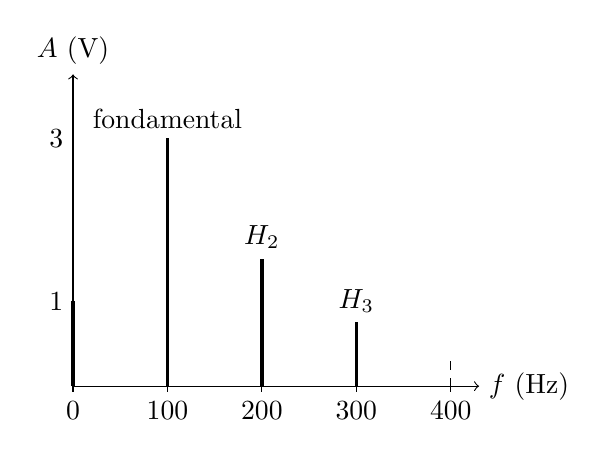
\begin{tikzpicture}[x=0.012cm,y=0.9cm]
  \draw[->] (0,0) -- (430,0) node[right] {$f$ (Hz)};
  \draw[->] (0,0) -- (0,4.4) node[above] {$A$ (V)};
  \draw[line width=1.2pt] (0,0) -- (0,1.2);
  \draw[line width=1.2pt] (100,0) -- (100,3.5);
  \draw[line width=1.2pt] (200,0) -- (200,1.8);
  \draw[line width=1.2pt] (300,0) -- (300,0.9);
  \draw[dashed] (400,0) -- (400,0.45);
  \foreach \x/\lab in {0/0,100/100,200/200,300/300,400/400}
    \draw (\x,0.08) -- (\x,-0.08) node[below] {\lab};
  \node[left] at (0,1.2) {$1$};
  \node[left] at (0,3.5) {$3$};
  \node[above] at (100,3.5) {fondamental};
  \node[above] at (200,1.8) {$H_2$};
  \node[above] at (300,0.9) {$H_3$};
\end{tikzpicture}
\end{center}

\paragraph{Exemple 1 — passage du temps vers le spectre.}
Soit
\[
s(t)=1+3\cos(2\pi\,100t)+1{,}8\cos(2\pi\,200t)+0{,}9\cos(2\pi\,300t).
\]
Le spectre comporte une raie de $\SI{1}{\volt}$ à $f=0$, une raie de $\SI{3}{\volt}$ à $\SI{100}{\hertz}$, une raie de $\SI{1.8}{\volt}$ à $\SI{200}{\hertz}$ et une raie de $\SI{0.9}{\volt}$ à $\SI{300}{\hertz}$.

\paragraph{Exemple 2 — passage du spectre vers le temps.}
Un spectre présente une composante continue de $\SI{2}{\volt}$, un fondamental de $\SI{4}{\volt}$ à $\SI{50}{\hertz}$ et une harmonique de rang 3 de $\SI{1}{\volt}$. Si les phases sont nulles :
\[
s(t)=2+4\cos(2\pi\,50t)+\cos(2\pi\,150t).
\]

\subsection{Action d'un filtre sur un spectre}\label{sec:elec-spectre-filtre}

Chaque raie du spectre d'entrée est multipliée par le module du filtre à la fréquence considérée :
\[
S_s(f)=|H(j2\pi f)|\,S_e(f).
\]
Ainsi, pour un filtre passe-bas de fréquence de coupure $f_c$, les raies situées très au-dessus de $f_c$ sont fortement atténuées, alors que les raies situées bien en dessous de $f_c$ sont pratiquement conservées.

\begin{center}
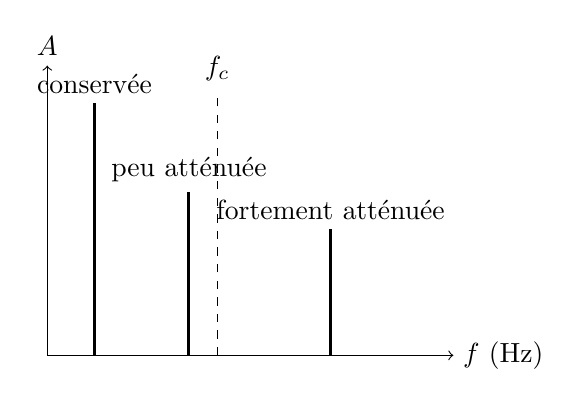
\begin{tikzpicture}[x=0.012cm,y=0.8cm]
  \draw[->] (0,0) -- (430,0) node[right] {$f$ (Hz)};
  \draw[->] (0,0) -- (0,4.6) node[above] {$A$};
  \draw[line width=1.1pt] (50,0) -- (50,4);
  \draw[line width=1.1pt] (150,0) -- (150,2.6);
  \draw[line width=1.1pt] (300,0) -- (300,2);
  \draw[dashed] (180,0) -- (180,4.2) node[above] {$f_c$};
  \node[above] at (50,4) {conservée};
  \node[above] at (150,2.6) {peu atténuée};
  \node[above] at (300,2) {fortement atténuée};
\end{tikzpicture}
\end{center}

\subsection{Gabarit d'un filtre}\label{sec:elec-gabarit-filtre}

Le gabarit traduit les exigences du cahier des charges dans le plan $(f,G_{\mathrm{dB}})$. Il distingue :
\begin{itemize}
  \item la bande passante, dans laquelle l'atténuation doit rester inférieure à $A_p$ ;
  \item la bande atténuée, dans laquelle l'atténuation doit être supérieure à $A_a$ ;
  \item la bande de transition, comprise entre $f_p$ et $f_a$.
\end{itemize}

\begin{center}
\begin{tikzpicture}[x=1.45cm,y=0.085cm]
  \draw[->] (0,0) -- (6.2,0) node[right] {$\log f$};
  \draw[->] (0,-66) -- (0,6) node[above] {$G_{\mathrm{dB}}$};
  \draw[dashed] (0,-3) -- (6,-3) node[right] {$-A_p$};
  \draw[dashed] (0,-40) -- (6,-40) node[right] {$-A_a$};
  \draw[dashed] (2.2,0) -- (2.2,-66) node[below] {$f_p$};
  \draw[dashed] (4.2,0) -- (4.2,-66) node[below] {$f_a$};
  \fill[pattern=north east lines,pattern color=gray] (0,-3) rectangle (2.2,-66);
  \fill[pattern=north east lines,pattern color=gray] (4.2,0) rectangle (6,-40);
  \draw[line width=1.2pt] (0,-0.5) -- (2.2,-2.5) .. controls (3.0,-7) and (3.7,-27) .. (4.2,-42) -- (6,-62);
  \node at (1.1,-12) {zone interdite};
  \node at (5.1,-18) {zone interdite};
  \node at (3.2,-12) {transition};
\end{tikzpicture}
\end{center}

Pour un passe-bas réel d'ordre $n$, la pente asymptotique dans la bande atténuée vaut approximativement
\[
-20n\ \text{dB/décade}.
\]
L'ordre minimal peut être estimé à partir du gabarit par
\[
n\geq \frac{A_a-A_p}{20\log_{10}(f_a/f_p)}.
\]
On retient l'entier immédiatement supérieur.

\paragraph{Exemple.}
On impose $A_p=\SI{3}{\decibel}$ à $f_p=\SI{100}{\hertz}$ et $A_a=\SI{40}{\decibel}$ à $f_a=\SI{1}{\kilo\hertz}$. Alors
\[
n\geq\frac{40-3}{20\log_{10}(1000/100)}=\frac{37}{20}=1{,}85.
\]
Il faut donc un filtre d'ordre au moins 2.

\subsection{Double filtre RC passe-bas}\label{sec:elec-double-filtre-rc}

Deux cellules RC passe-bas mises en cascade ne peuvent être multipliées directement que si la seconde cellule ne charge pas la première, par exemple grâce à un suiveur entre les deux cellules.

\begin{center}
\begin{circuitikz}[american voltages]
  \draw
  (0,0) node[left] {$u_e$}
    to[R,l=$R_1$] (2,0) coordinate (A)
    to[short] (2.8,0)
    node[draw,minimum width=1.2cm,minimum height=.8cm] (B) {suiveur}
    (B.east) to[R,l=$R_2$] (5.2,0) coordinate (C)
    to[short] (6,0) node[right] {$u_s$};
  \draw (A) to[C,l_=$C_1$] (2,-2) node[ground]{};
  \draw (C) to[C,l_=$C_2$] (5.2,-2) node[ground]{};
\end{circuitikz}
\end{center}

Avec découplage parfait :
\[
H(p)=H_1(p)H_2(p)
=\frac{1}{(1+R_1C_1p)(1+R_2C_2p)}.
\]
Si les deux cellules sont identiques, $R_1=R_2=R$ et $C_1=C_2=C$ :
\[
H(p)=\frac{1}{(1+RCp)^2}.
\]
Le filtre est d'ordre 2. Sa pente asymptotique en haute fréquence vaut $-40$ dB/décade. À la fréquence $f_c=1/(2\pi RC)$ de chaque cellule, le module total vaut
\[
|H(j\omega_c)|=\left(\frac{1}{\sqrt{2}}\right)^2=\frac12,
\]
soit un gain de $-6$ dB.

\paragraph{Attention au chargement.}
Sans suiveur, la deuxième cellule modifie la première : la fonction de transfert n'est plus le simple produit des deux fonctions de transfert élémentaires. Il faut alors écrire les équations du circuit complet.

\subsection{Spectre d'un signal échantillonné et repliement}\label{sec:elec-repliement-spectre}

L'échantillonnage à la fréquence $f_e$ répète le spectre du signal analogique autour de chaque multiple de $f_e$ :
\[
\ldots,-2f_e,-f_e,0,f_e,2f_e,\ldots
\]
Si le signal contient une fréquence maximale $f_{\max}$, les copies ne se recouvrent pas lorsque
\[
f_e>2f_{\max}.
\]
Dans le cas contraire, elles se superposent : c'est le repliement de spectre.

\begin{center}
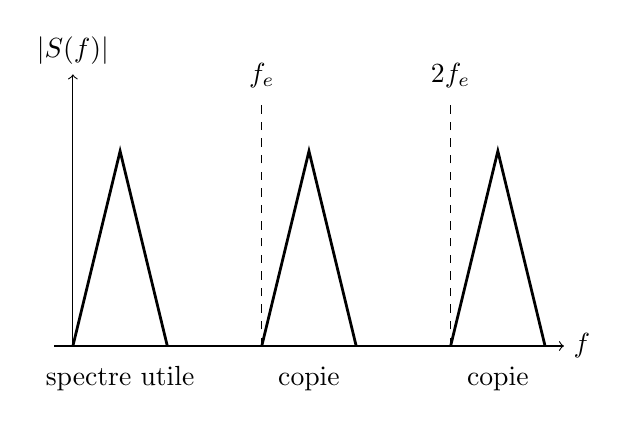
\begin{tikzpicture}[x=0.012cm,y=0.75cm]
  \draw[->] (-20,0) -- (520,0) node[right] {$f$};
  \draw[->] (0,0) -- (0,4.6) node[above] {$|S(f)|$};
  \foreach \c in {0,200,400}{
    \draw[line width=1pt] (\c,0) -- (\c+50,3.3) -- (\c+100,0);
  }
  \draw[dashed] (200,0) -- (200,4.2) node[above] {$f_e$};
  \draw[dashed] (400,0) -- (400,4.2) node[above] {$2f_e$};
  \node at (50,-0.55) {spectre utile};
  \node at (250,-0.55) {copie};
  \node at (450,-0.55) {copie};
\end{tikzpicture}
\end{center}

\paragraph{Exemple de fréquence repliée.}
Un sinus de fréquence $f=\SI{1.4}{\kilo\hertz}$ est échantillonné à $f_e=\SI{2}{\kilo\hertz}$. La fréquence observée dans la bande $[0,f_e/2]$ est
\[
f_{\mathrm{alias}}=|f_e-f|=\SI{0.6}{\kilo\hertz}.
\]
Le système numérique confond donc une composante à $\SI{1.4}{\kilo\hertz}$ avec une composante à $\SI{600}{\hertz}$.

\subsection{Filtre anti-repliement}\label{sec:elec-filtre-anti-repliement}

Le filtre anti-repliement est un filtre passe-bas analogique placé avant le CAN. Il doit :
\begin{itemize}
  \item conserver la bande utile jusqu'à $f_{\max}$ ;
  \item atténuer suffisamment les composantes situées au voisinage et au-delà de $f_e/2$ ;
  \item respecter un gabarit défini par $f_p=f_{\max}$ et une fréquence atténuée au plus tard à $f_a=f_e/2$.
\end{itemize}

\begin{center}
\begin{tikzpicture}[x=1.45cm,y=0.085cm]
  \draw[->] (0,0) -- (6.2,0) node[right] {$\log f$};
  \draw[->] (0,-66) -- (0,5) node[above] {$G_{\mathrm{dB}}$};
  \draw[dashed] (2.2,0) -- (2.2,-65) node[below] {$f_{\max}$};
  \draw[dashed] (4.4,0) -- (4.4,-65) node[below] {$f_e/2$};
  \draw[dashed] (0,-40) -- (6,-40) node[right] {$-A_a$};
  \draw[line width=1.2pt] (0,-0.5) -- (2.2,-2) .. controls (3.0,-6) and (3.8,-25) .. (4.4,-42) -- (6,-62);
  \node at (1.2,-10) {bande utile};
  \node at (3.3,-12) {transition};
  \node at (5.15,-20) {bande atténuée};
\end{tikzpicture}
\end{center}

Le choix de $f_e$ ne se limite donc pas à l'inégalité de Shannon-Nyquist : une marge est nécessaire pour laisser au filtre analogique une bande de transition réalisable.
